%  LaTeX support: latex@mdpi.com
%  In case you need support, please attach all files that are necessary for compiling as well as the log file, and specify the details of your LaTeX setup (which operating system and LaTeX version / tools you are using).

% You need to save the "mdpi.cls" and "mdpi.bst" files into the same folder as this template file.

%==============

\documentclass[information,article,submit,moreauthors,Latex,dvi2pdf,10pt,a4paper]{Definitions/mdpi}

%--------------------
% Class Options:
%--------------------
% journal
%----------
% Choose between the following MDPI journals:
% actuators, admsci, aerospace, agriculture, agronomy, algorithms, animals, antibiotics, antibodies, antioxidants, applsci, arts, atmosphere, atoms, axioms, batteries, behavsci, beverages, bioengineering, biology, biomedicines, biomimetics, biomolecules, biosensors, brainsci, buildings, carbon, cancers, catalysts, cells, challenges, chemosensors, children, chromatography, climate, coatings, computation, computers, condensedmatter, cosmetics, cryptography, crystals, data, dentistry, designs, diagnostics, diseases, diversity, econometrics, economies, education, electronics, energies, entropy, environments, epigenomes, fermentation, fibers, fishes, fluids, foods, forests, futureinternet, galaxies, games, gels, genealogy, genes, geosciences, geriatrics, healthcare, horticulturae, humanities, hydrology, informatics, information, infrastructures, inorganics, insects, instruments, ijerph, ijfs, ijms, ijgi, inventions, jcdd, jcm, jdb, jfb, jfmk, jimaging, jof, jintelligence, jlpea, jmse, jpm, jrfm, jsan, land, languages, laws, life, literature, lubricants, machines, magnetochemistry, marinedrugs, materials, mathematics, mca, mti, medsci, medicines, membranes, metabolites, metals, microarrays, micromachines, microorganisms, minerals, molbank, molecules, mps, nanomaterials, ncrna, neonatalscreening, nutrients, particles, pathogens, pharmaceuticals, pharmaceutics, pharmacy, philosophies, photonics, plants, polymers, processes, proteomes, publications, recycling, religions, remotesensing, resources, risks, robotics, safety, sensors, separations, sexes, sinusitis, socsci, societies, soils, sports, standards, sustainability, symmetry, systems, technologies, toxics, toxins, universe, urbansci, vaccines, vetsci, viruses, water
%---------
% article
%---------
% The default type of manuscript is article, but can be replaced by:
% addendum, article, book, bookreview, briefreport, casereport, changes, comment, commentary, communication, conceptpaper, correction, conferencereport, expressionofconcern, meetingreport, creative, datadescriptor, discussion, editorial, essay, erratum, hypothesis, interestingimage, letter, newbookreceived, opinion, obituary, projectreport, reply, retraction, review, sciprints, shortnote, supfile, technicalnote
% supfile = supplementary materials
%----------
% submit
%----------
% The class option "submit" will be changed to "accept" by the Editorial Office when the paper is accepted. This will only make changes to the frontpage (e.g. the logo of the journal will get visible), the headings, and the copyright information. Also, line numbering will be removed. Journal info and pagination for accepted papers will also be assigned by the Editorial Office.
%------------------
% moreauthors
%------------------
% If there is only one author the class option oneauthor should be used. Otherwise use the class option moreauthors.
%---------
% pdftex
%---------
% The option pdftex is for use with pdfLaTeX. If eps figure are used, remove the option pdftex and use LaTeX and dvi2pdf.

%=================================================================
\firstpage{1}
\makeatletter
\setcounter{page}{\@firstpage}
\makeatother
\pubvolume{xx}
\issuenum{1}
\articlenumber{5}
\pubyear{2018}
\copyrightyear{2018}
%\externaleditor{Academic Editor: name}
\history{Received: date; Accepted: date; Published: date}
%\updates{yes} % If there is an update available, un-comment this line

%------------------------------------------------------------------
% The following line should be uncommented if the LaTeX file is uploaded to arXiv.org
%\pdfoutput=1

%=================================================================
% Add packages and commands here. The following packages are loaded in our class file: fontenc, calc, indentfirst, fancyhdr, graphicx, lastpage, ifthen, lineno, float, amsmath, setspace, enumitem, mathpazo, booktabs, titlesec, etoolbox, amsthm, hyphenat, natbib, hyperref, footmisc, geometry, caption, url, mdframed

\usepackage{array}
\usepackage{multirow}
\usepackage{pbox}
\usepackage{arydshln}
\usepackage{dirtytalk}
\usepackage{xcolor}
\usepackage{soul}
\usepackage[skins]{tcolorbox}
\usepackage{ulem}
\tcbset{commonstyle/.style={boxrule=0pt,sharp corners,notitle,enhanced jigsaw,nobeforeafter,boxsep=0pt}}
\newtcolorbox{mycolorbox}[1][]{commonstyle,#1}

%=================================================================
% Full title of the paper (Capitalized)
\Title{Quantifying Bicycle Network Connectivity in Lisbon using Open Data $^\dagger$}

% Author Orchid ID: enter ID or remove command
\newcommand{\orcidauthorA}{0000-0003-0554-734X} % Add \orcidA{} behind the author's name

% Authors, for the paper (add full first names)
\Author{Lorena Abad $^{*}$ \orcidA{} and Lucas van der Meer}
% Authors, for metadata in PDF
\AuthorNames{Lorena Abad and Lucas van der Meer}

% Affiliations / Addresses (Add [1] after \address if there is only one affiliation.)
\address{NOVA Information Management School (NOVA-IMS), Universidade Nova de Lisboa, Campus de Campolide, 1070-032, Lisbon, Portugal; lore.abad6@gmail.com (L.A.); luukvandermeer@live.nl (L.M.)}

% Contact information of the corresponding author
\corres{Correspondence: lore.abad6@gmail.com}

% Current address and/or shared authorship
\firstnote{This paper is an extended version of our \colorbox{green}{\sout{paper published} presentation} in the workshop ``Open Data for Open Cities V~2.0'', Lund, Sweden, 12 June 2018. \colorbox{green}{\cite{OD4OC}}}

% Simple summary
%\simplesumm{}

% Abstract (Do not use inserted blank lines, i.e. \\)
\abstract{Stimulating non-motorized transport has been a key point on sustainable mobility agendas for cities around the world. Lisbon is no exception, as it invests in the implementation of new bike infrastructure. Quantifying the connectivity of such a bicycle network can help evaluate its current state and highlight specific challenges that should be addressed. Therefore, the aim of this study is to develop an exploratory score that allows a quantification of the bicycle network connectivity in Lisbon based on open data. For each part of the city, a score was computed based on how many common destinations (e.g. schools, universities, supermarkets, hospitals) were located within an acceptable biking distance when using only bicycle lanes and roads with low traffic stress for cyclists. Taking a weighted average of these scores resulted in an overall score for the city of Lisbon of only 8.6 out of 100 points. This shows, at a glance, that the city has still a long way to go before achieving their objectives regarding bicycle use in the city.}


% Keywords
\keyword{bicycle network analysis; levels of traffic stress; sustainable mobility; open data; bicycle network connectivity; BNA score}

% The fields PACS, MSC, and JEL may be left empty or commented out if not applicable
%\PACS{J0101}
%\MSC{}
%\JEL{}

% If this is an expanded version of a conference paper, please cite it here: enter the full citation of your conference paper, and add $^\S$ in the end of the title of this article.
%\conference{}

%%%%%%%%%%%%%%%%%%%%%%%%%%%%%%%%%%%%%%%%%%
% Only for the journal Data:

%\dataset{DOI number or link to the deposited data set in cases where the data set is published or set to be published separately. If the data set is submitted and will be published as a supplement to this paper in the journal Data, this field will be filled by the editors of the journal. In this case, please make sure to submit the data set as a supplement when entering your manuscript into our manuscript editorial system.}

%\datasetlicense{license under which the data set is made available (CC0, CC-BY, CC-BY-SA, CC-BY-NC, etc.)}

%%%%%%%%%%%%%%%%%%%%%%%%%%%%%%%%%%%%%%%%%%
\begin{document}

%%%%%%%%%%%%%%%%%%%%%%%%%%%%%%%%%%%%%%%%%%
%% Sections that are not mandatory are listed as such. The section titles given are for Articles. Review papers and other article types have a more flexible structure.

%% Only for the journal Gels: Please place the Experimental Section after the Conclusions

%%%%%%%%%%%%%%%%%%%%%%%%%%%%%%%%%%%%%%%%%%
\section{Introduction}

Stimulating non-motorized transport has been one of the many strategies adopted by cities to tackle climate change \cite{Banister2011} and boost their inhabitants' living conditions.
\begin{mycolorbox}[colback=cyan]
Introducing sustainable mobility into an urban planning agenda has beneficial effects on public health, as it decreases air pollution and stimulates physical activity \cite{Fraser2011,DeHartog2010,Torres2018,Carley2017,Bopp2018}. \sout{It is not only a way to improve our environment, by decreasing air pollution and energy consumption \cite{Fraser2011}; but also to ameliorate citizens' health \cite{DeHartog2010},}
\end{mycolorbox}
\colorbox{cyan}{Additionally, it has proven to} reduce traffic jams \cite{Kosha2016} and reactivate public spaces \cite{DeManuelJerez2016}. Therefore, investing in cycling and pedestrian infrastructure is a critical part of transportation policies in metropolitan areas.

The city of Lisbon has undertaken this investment by establishing new cycle ways and \colorbox{cyan}{public} bike-sharing stations, \colorbox{cyan}{i.e. \textit{\href{https://www.gira-bicicletasdelisboa.pt/}{Gira Bicicletas}}}. The municipality hopes to turn the bicycle into a means of transport that, along with public transportation, will enable inhabitants to make safe and efficient short distance journeys, up to six kilometers, \colorbox{cyan}{without the use of private transport \lucas[aren't bicycles private transport?] \cite{CamaraMunicipaldeLisboa,Marrana2018}}. This is happening in a city where 89\% of commuters use a private vehicle \cite{CamaraMunicipaldeLisboa2016}, with a car occupancy of 1.2 passengers per vehicle \cite{Silva2017}. The municipality originally presented a plan which would introduce 200 km of \lucas[new?] cycle ways (Fig. \ref{fig1}) into the city's infrastructure by 2018 \cite{Susete2016}. However, by early 2018, only 80 km of the proposed routes had actually been built. The planned completion date has been pushed back to 2020 \cite{Andre2018}.

\begin{figure}[ht]
	\begin{center}
		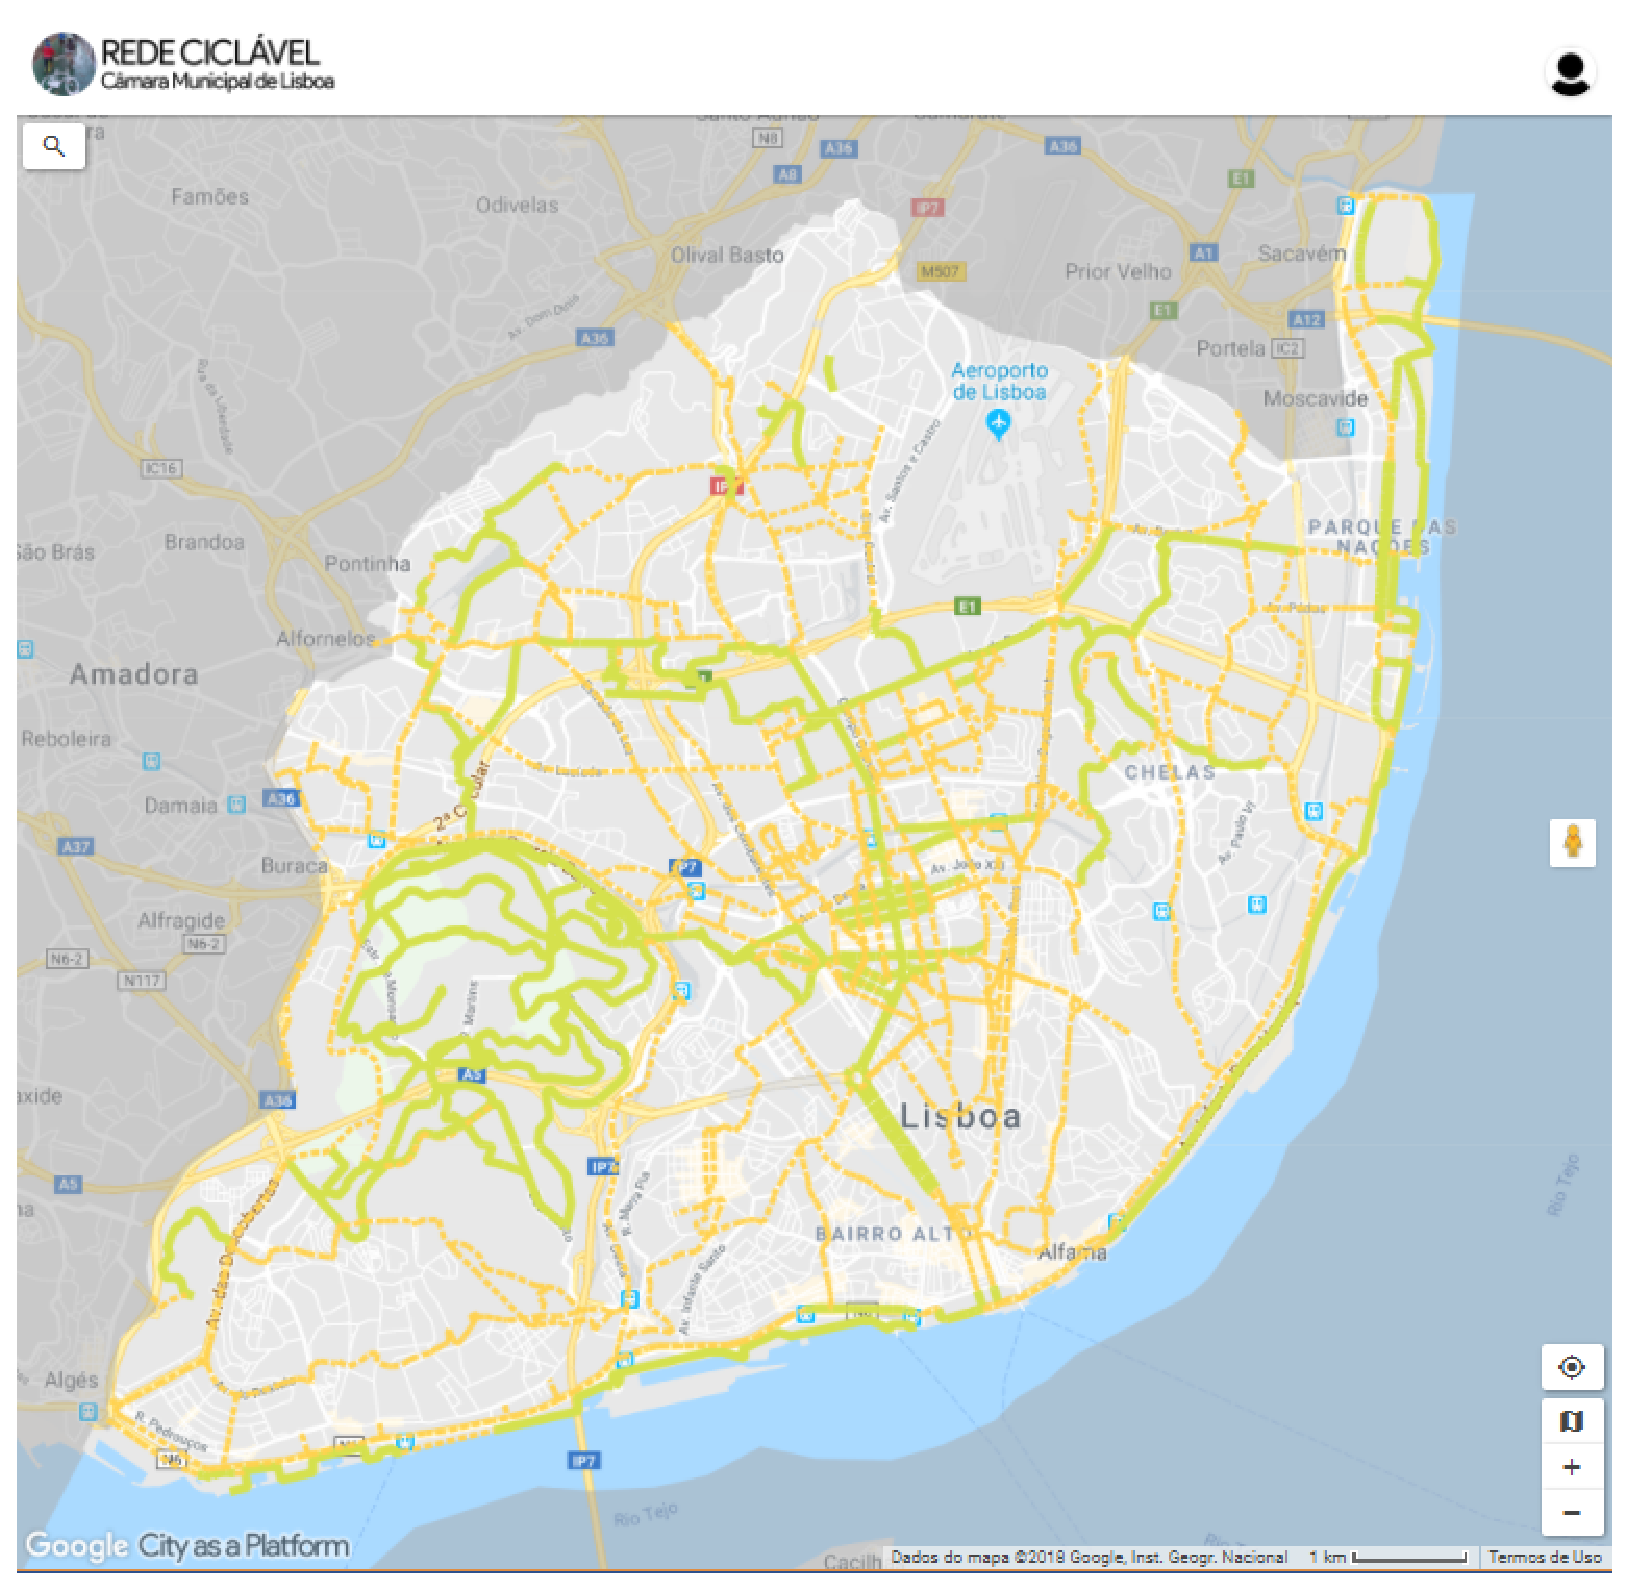
\includegraphics[height=8.5cm]{fig1}
		\caption{Existing (green) and proposed (dashed yellow) biking infrastructure according to the Lisbon City Council.} Source: \protect\href{https://lisboa.city-platform.com/app/?a=redeciclavel}{City as a Platform}.
		\label{fig1}
	\end{center}
\end{figure}

In the meantime, Lisbon's cyclists have increased in number \cite{Baratto2016}, which intensifies the need to invest in well-connected and safe infrastructure, not only for regular commuter trips, but also for trips to common destinations (e.g. schools, universities, supermarkets, hospitals). Quantifying the bicycle network's connectivity can help city officials to evaluate its current state and identify specific challenges that should be addressed. The use of publicly available data sources should be favored for such inquiries, given their ease of access, constant updates, reproducibility, and knowledge sharing boost\lucas[?] \cite{opendatahandbook,EuropeanDataPortal2018}. Therefore, the aim of this study is to develop an exploratory score that allows a quantification of the bicycle network connectivity in Lisbon based on open data, as a first attempt to apply such an index to a European city with a developing biking infrastructure.

The remainder of this paper will be structured as follows:
\begin{mycolorbox}[colback=yellow]
Section \ref{background} provides an overview of related work and the state of the art regarding bicycle network connectivity \lucas[sounds funny]. Section \ref{pfb} describes the specific approach on which this study is based.
\end{mycolorbox}
Section \ref{methods} details the adapted methodology applied to address the particular case of the Lisbon study area. Section \ref{results} presents the main results, discusses them within the context of Lisbon, and compares them to other cities' examples. Section \ref{conclusion} concludes the report and summarizes its limitations and finally, section \ref{future} suggests directions for future research and development.

\section{Background} \label{background}

Bicycle network analyses have been undertaken from several angles, making use of GIS tools \cite{Manum2013,Cooper2017}.

\begin{mycolorbox}[colback=yellow]
Connectivity analyses and measures have been developed and applied to understand how accessible a city's bike infrastructure really is (see Chapter 3 of \cite{Twadell2018} for an overview of these methods).
\end{mycolorbox}

A recurrent approach within the literature is

\begin{mycolorbox}[colback=yellow]
\sout{the level of traffic stress (LTS). Mekuria, Furth \& Nixon proposed a scheme to classify the road segments in four LTS, ranging from LTS 1, – the level suitable for children - to 4 – the level tolerated by the strong and fearless cyclists.}
the quantification of cyclists' percieved traffic stress \cite{Sorton1994,Geller2006}. Mekuria, Furth \& Nixon \cite{Mekuria2012b} proposed a scheme to classify road segments into four levels of traffic stress (LTS), ranging from LTS 1, the level suitable for children; to LTS 4, the level tolerated by “strong and fearless” cyclists \cite{Dill2016}. Their approach was tested via \sout{an analysis of the network connectivity with a thorough review of every segment and crossing, allowing an integral characterization of the bike network and assigning each section a stress level.} a case study in San Diego, California, in which every street and crossing was classified by LTS. In later work, Furth, Mekuria \& Nixon \cite{Furth2016} developed a measure for the connectivity of low stress cycling networks, using origin-destination data from home-to-work trips. Applying their methodology once again in San Diego, California, they concluded that the road network is divided into disconnected islands of low-stress segments. Investments in new bicycle infrastructure between such islands could drastically improve the connectivity of low-stress networks.

Building on the findings of \cite{Mekuria2012b}, Lowry et al. \cite{Lowry2016} created a tool for transportation planners to rank more than 750 bicycle improvement projects from the Seattle, Washington’s Bicycle Master Plan, based on their potential to connect homes and important destinations over a low-stress network. The same master plan was evaluated in \cite{Lowry2017}, by comparing the bicycle network connectivity for different types of cyclists and different neighborhoods in Seattle, in both the existing and proposed situation. The results showed that connectivity differs between neighborhoods and types of cyclists, and emphasized the importance of policies and programs that increase the confidence of cyclists. Both \cite{Lowry2016} and \cite{Lowry2017} focused solely on utilitarian travel, and did not distinguish between destinations of varying importance.

Boettge et al. \cite{Boettge2017} validated the LTS concept in a qualitative way, gathering information from individual cyclists using surveys. Their findings in St. Louis, Missouri, confirmed a positive correlation between cyclists' levels of stress on a road and the speed limit, number of lanes and functional class of the road. No relationship was found between specific bicycle facilities and LTS.
\end{mycolorbox}

\section{PeopleForBikes \textquotedblleft Bike Network Analysis score\textquotedblright approach} \label{pfb}

\begin{mycolorbox}[colback=yellow]
Yet another example of the use of LTS to quantify bicycle network connectivity comes from the organization \href{https://peopleforbikes.org/}{PeopleForBikes} (PfB). They developed a scoring system called the \textit{Bike Network Analysis score} (BNA score). BNA is a slightly modified version of LTS whose methodology is described by \cite{Mekuria2012b}.
\end{mycolorbox}
\begin{mycolorbox}[colback=cyan]
The modifications add bicycle facility types that were not considered by the initial LTS approach. Besides this, the approach is the same, classifying the four original LTS levels into Low Stress (LTS 1 and LTS 2) and High Stress (LTS 3 and LTS 4).
\end{mycolorbox}
The BNA score determines how people in a city can get to common destinations on a comfortable and connected bike network.
\begin{mycolorbox}[colback=yellow]
The way these destinations are picked is similar to how Lowry et al. define their so called \textit{basket of destination types}, following the theory that \say{it is possible that some bicyclists would not need certain destinations in the basket, and it is also possible that different bicyclists would have unique preferences for particular destination types, e.g. preference for a particular restaurant. Nevertheless, (\ldots) the concept of a basket provides a means to calculate a meaningful metric with objectivity} \cite[p.130]{Lowry2016}.
\end{mycolorbox}
The score is computed by counting the total number of common destination points accessible within 10 minutes on a low-stress bike network from an origin census block. A scoring scale between 0 and 100 is assigned to each destination type, in a stepped manner\lucas{not sure what that means}. Finally, the scores for all census blocks are aggregated as a weighted averaged to get to one score for the whole city \cite{PeopleforBikes2014}.

\begin{mycolorbox}[colback=yellow]
\sout{PeopleForBikes targets USA cities and towns, basing their analysis mainly on OpenStreetMap and US Census data.} The PfB analysis is unique because the methodology is based on OpenStreetMap (OSM), a crowd-sourced project to create a free and editable map of the entire world. The use of OSM, although complemented by open governmental data from the 2011 US Census, still makes the tool easier to implement in other areas where street network and points of interest information might not be available to the public.
\end{mycolorbox}

Therefore, this paper used the PeopleForBikes \href{https://github.com/azavea/pfb-network-connectivity}{open source} methodology as a guide to develop a BNA score for the city of Lisbon.

\section{Data and methods} \label {methods}

\subsection{Data acquisition and preprocessing} \label{data}

The computation of the BNA score for Lisbon in this paper is based solely on open data. The main sources used were OpenStreetMap (OSM), Lisbon Municipal Council's Spatial Open Data and Open Data Portal, and the National Statistics Institute.

The OSM data was downloaded in February 2018 through the built-in QGIS tool and loaded into a PostgreSQL database in two formats: the \textit{osm2pgrouting} bicycle map
configuration .XML file to generate edge/segment and node/intersection tables, and the \textit{osm2pgsql} adjusted to the .STYLE file from PeopleForBikes\lucas{<- Not sure what you're trying to say here} to generate points, lines, and polygon base data.

The \href{http://geodados.cm-lisboa.pt/}{CML data} consisted of Lisbon's Council \lucas{I haven't seen this term "Council" used in reference to geographical area. Maybe say Lisbon's city/municipal boundary or Lisbon's metropolitan area instead} outline, the Parishes belonging to the Council, and the existing cycleways. The Parishes data was merged with corresponding population obtained from the \href{http://censos.ine.pt/}{2011 Portuguese Census}.

The PeopleForBikes methodology uses census blocks as the unit of analysis.
\begin{mycolorbox}[colback=yellow]
\sout{As this information was not available for the study area, a hexagonal grid overlying Lisbon Council was generated to perform the network analysis on a smaller scale, allowing a local evaluation of the resulting stress network.} However, information at this administrative level was not available for the study area. Therefore, a hexagonal grid was laid over the Lisbon Council to perform the analysis at a higher spatial resolution and evaluate the results locally. A hexagonal shape was selected over a rectangular grid as it reduces the bias of the edge-effect generating a more symmetrical neighborhood and is thus more convenient for connectivity analyses \cite{Birch2007}.
\end{mycolorbox}
Each hexagon in the grid had an x-spacing of 200 m. This value was arbitrarily chosen, but based on the underlying idea that all destinations in a single cell should be within a reasonable walking distance of each other. The population of each cell was estimated from the parish population data, by simply dividing the total population of a parish by the number of grid cells that belong predominantly to that parish.

For the pre-processing, all the data were projected to ETRS89 / Portugal TM06 and clipped to the study area outline. Next, the point and polygon data were organized to create one homogeneous layer with common destination points. The centroids of the polygon data were calculated to be appended to the point data. For polygons that comprehended large areas (nature reserves and parks), a spatial join with the hexagonal grid was performed to assign a destination to each cell centroid that intersects these polygons.

Finally, the segment data were built upon attributes like maximum speed, number of lanes, road type, taken from OSM tags. To assure that the official cycleways in the CML data were comprised within the OSM segments, an intersection between them was performed. An additional variable concerning the mean slope was added for this analysis, given the challenging conditions of the study area. It was calculated for each segment from the Digital Terrain Model raster (49 m resolution), obtained from the \href{http://dados.cm-lisboa.pt}{Open Data Portal}.

\subsection{Biking Network Stress Levels classification} \label{classification}

The segment data were categorized into two possible classes: low and high stress. This classification follows the PeopleForBikes simplification of the LTS mentioned in section \ref{pfb}. The conditions to determine if a segment is of high or low stress are based on five variables: maximum speed, whether or not it is a residential area, the number of lanes, the slope, and a bicycle tag existing among the OSM information. With these variables, the type of segments, identified by the OSM tag are classified. The criteria followed can be found in Table \ref{table1}.

\begin{table}[H]
	\begin{center}
    	\small
		\centering
		\caption{Classification criteria for stress level segment labeling.}
		\label{table1}

\begin{tabular}{m{3.2cm} >{\centering}m{2cm} >{\centering}m{2cm} >{\centering}m{2cm} >{\centering}m{1.3cm} >{\centering}m{1.cm} >{\centering}m{1.7cm} @{}m{0pt}@{}}
			\hline
			\centering Type of segment &
			\centering Maximum speed &
			\centering Residential area &
			\centering Number of lanes &
			\centering Slope &
			\centering Bicycle tag &
			\centering Stress Level \tabularnewline
			\hline \tabularnewline [-5pt]
			\raggedright Municipality designated cycleway & -------- & -------- & -------- & -------- & -------- & Low &  \tabularnewline [15pt]
			\hdashline \tabularnewline [-5pt]
			OSM tagged cycleway & -------- & -------- & -------- & -------- & -------- & Low & \tabularnewline [15pt]
			\hdashline \tabularnewline [-5pt]
			\multirow{3}{3cm}{Shared lanes} & $\mathbf{\leq}$35 km/h & Yes & -------- & -------- & -------- & Low & \tabularnewline[15pt]
			& $\mathbf{\leq}$35 km/h & No & 1 & $\mathbf{<}$10\% & -------- & Low & \tabularnewline [15pt]
			& $\mathbf{>}$35 km/h & No & -------- & -------- & -------- & High & \tabularnewline [15pt]
			\hdashline \tabularnewline [-5pt]
			\multirow{4}{3cm}{Motorized road network (road, primary, secondary and tertiary segments and links)} & $\mathbf{\geq}$50 km/h & No & $\mathbf{>}$1 & -------- & -------- & High & \tabularnewline [10pt]
			& \pbox{3cm}{$\mathbf{\geq}$50 km/h \\ $\mathbf{<}$60 km/h} & No & 1 & $\mathbf{<}$10\% & -------- & Low & \tabularnewline [20pt]
			& \pbox{3cm}{$\mathbf{\geq}$50 km/h \\ $\mathbf{<}$60 km/h} & No & 1 & $\mathbf{>}$10\% & -------- & High & \tabularnewline [20pt]
			& $\mathbf{\leq}$30 km/h & No & 1 & $\mathbf{<}$10\% & -------- & Low & \tabularnewline [10pt]
			\hdashline \tabularnewline [-5pt]
			\multirow{2}{3cm}{Residential roads (unclassified, residential, living street)} & $\mathbf{>}$40 km/h & -------- & -------- & -------- & -------- & High & \tabularnewline [15pt]
			& $\mathbf{\leq}$40 km/h & -------- & -------- &  $\mathbf{<}$10\% & -------- & Low & \tabularnewline [20pt]
			\hdashline \tabularnewline [-5pt]
			\raggedright Pedestrian segments and foot ways & -------- & -------- & -------- & -------- & -------- & High & \tabularnewline [10pt]
			\hdashline \tabularnewline [-5pt]
			\raggedright Roundabouts segments without bike path & -------- & -------- & -------- & -------- & -------- & High & \tabularnewline [10pt]
			\hdashline \tabularnewline [-5pt]
			\multirow{2}{3cm}{Service lanes (public transport)} & $\mathbf{\leq}$30 km/h & -------- & -------- & $\mathbf{<}$10\% & -------- & Low & \tabularnewline [10pt]
			& $\mathbf{>}$30 km/h & -------- & -------- &  -------- & -------- & High & \tabularnewline [10pt]
			\hdashline \tabularnewline [-5pt]
			Paths & -------- & -------- & -------- & -------- & -------- & Low & \tabularnewline [10pt]
			\hdashline \tabularnewline [-5pt]
			Tracks & -------- & -------- & -------- & -------- & -------- & High & \tabularnewline [10pt]
			\hdashline \tabularnewline [-5pt]
			\multirow{3}{3cm}{Remaining unclassified segments} & -------- & -------- & -------- & $\mathbf{>}$10\% & -------- & High & \tabularnewline [15pt]
			& -------- & -------- & -------- & -------- & \pbox{4cm}{Yes \\ Designated \\ Destination} & Low & \tabularnewline[30pt]
			& -------- & -------- & -------- & -------- & \pbox{4cm}{No \\ Dismount} & High & \tabularnewline [20pt]
			\hline
		\end{tabular}
	\end{center}
\end{table}

\bigskip

\subsection{Bike Network Analysis (BNA)} \label{bna}

A network analysis was performed to count, for each cell separately, the number of destinations reachable within a biking distance of six kilometers on the low stress network. First, the hexagonal grid and destinations were spatially joined, so that the number of destinations per type was known for each cell. A spatial join was also performed between the grid and the nodes of the low-stress network, to select only those cells that are reachable with the low-stress network. For each of these, the centroid was computed, after which the nearest node to each centroid was found (Figure \ref{fig2}). By doing this, each reachable cell was now represented by one single node.

\begin{figure}[ht!]
	\begin{center}
		\captionsetup{justification=centering}
		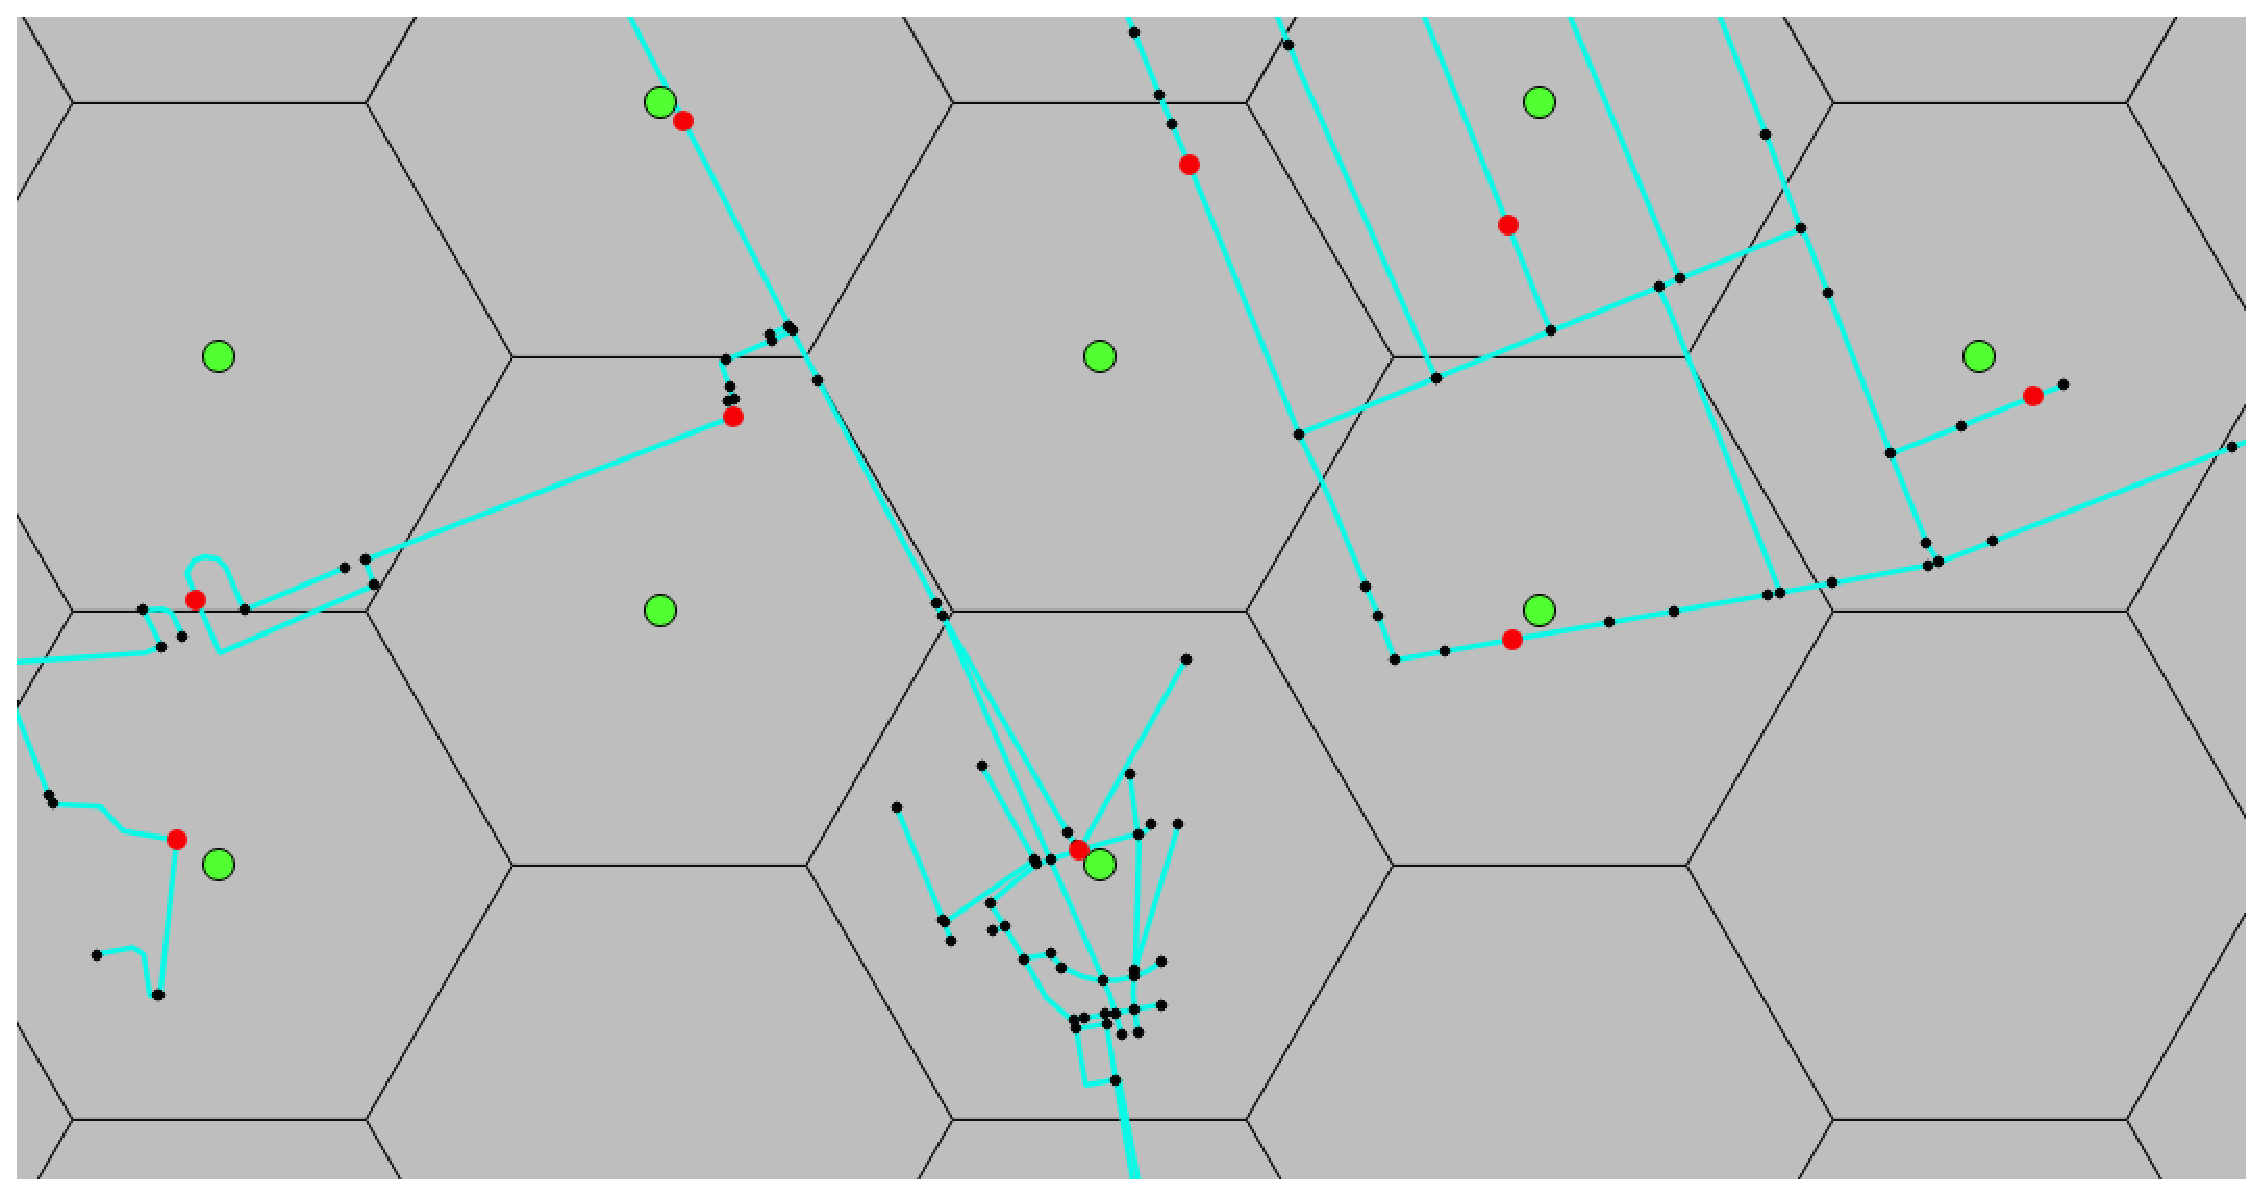
\includegraphics[height=5cm]{fig2}
		\caption{Nearest node selection. The low-stress network consists of the blue lines (edges) and black dots (nodes). The green dots represent the cell centroids. The nearest nodes to each of the cell centroids are colored red. }
		\label{fig2}
	\end{center}
\end{figure}

Shortest paths were computed between all the nearest nodes, using the Dijkstra algorithm. Only those that were shorter than six kilometers were kept. Knowing that each node uniquely represents a grid cell, for each cell it was now known which other cells were reachable by the low-stress network within the six kilometers buffer. Combining this information with the destination counts, the number of reachable destinations of each type for each cell could be determined. These data were used as input for the calculation of the BNA scores.

\subsection{BNA scoring} \label{score}

Each cell on the hexagonal grid was evaluated according to its capacity to reach the destinations within the study area, being able to get a maximum score of 100 points. These destinations were not equally weighted, given that, their number and importance differ from one another. For example, universities are not as common as parks, therefore the ability of the network to reach one park would be rewarded with 30 points whereas reaching a university campus or building would award the cell 70 points. Hence, different scoring processes were established for each type of destination, which can be observed in Table \ref{table2}.


\begin{table}[ht]
	\begin{center}
       	\small
		\centering
		\caption{Methodology for scoring destinations.}
		\label{table2}

		\begin{tabular}{m{1.2cm} m{6.7cm} b{6.5cm}}
		\hline
		\centering Scoring process &
		\centering Criteria &
		\centering General methodology \tabularnewline
		\hline \\ [-5pt]
		\centering A &
		\centering \pbox{6.7cm}{First low stress destination = 30 points \\ Second low stress destination = 20 points \\ Third low stress destination = 20 points} &
		\centering \multirow{3}{6.5cm}{\pbox{6.5cm}{The maximum amount of points is 100.\\ The points are given in a cumulative form, considering the number of destinations that the low stress network allows to reach within a biking distance of 6 km. \\ If all the destinations can be reached, then 100 points are granted. \\ If more destinations can be reached than defined in the criteria on the left, extra points are given based on a ratio: \\ No. of extra destinations that can be reached by the low stress network / total number of extra destinations within a distance of 6 km,represented by a circular buffer around the concerned node.}}
		\tabularnewline[35pt]
		\centering B &
		\centering \pbox{6.7cm}{First low stress destination = 40 points \\ Second low stress destination = 20 points \\ Third low stress destination = 10 points} &
		\tabularnewline[30pt]
		\centering C &
		\centering First low stress destination = 70 points   &\tabularnewline[30pt]
		\centering D &
		\centering \pbox{6.7cm}{First low stress destination = 60 points \\ Second low stress destination = 20 points} &\tabularnewline [10pt]
		\hline
	\end{tabular}
\end{center}
\end{table}

The scores for each type of destination, following the scoring process described in Table \ref{table2}, are then categorized into three distinct groups: Opportunity for those destinations related to education, Core Services for health, consumer goods, and social services, and Recreation including parks and nature reserves. Within each of these categories, the scores for the different types of destinations are given a weight (Table \ref{table3}) that will allow the calculation of a weighted average per category. Finally, these averaged scores are once again aggregated given the weights assigned to the categories, and the BNA score per cell is obtained. To calculate the overall score for the whole study area, a final weighted average is performed. This average consists on the addition of all the cells within the grid, weighted by the fraction of the population they would comprehend, assuming that the population is equally distributed along each parish.

The complete scoring process can best be summarized using a short example. Assume in a radius of 6 km around a cell there are 5 parks and 2 nature reserves. With the low stress network, one can reach 4 of these parks and 1 nature reserve. Both parks and nature reserves have scoring process A, so for the first park and the nature reserve, the cell will get 30 points. The fact that a second and third park can be reached, will account for two times 20 points more. Hence, for three reachable parks the cell has now got 70 points. There are two more parks in the radius, of which one can be reached. That is, of the remaining 30 points (100-70), the cell will get half, i.e. 15 points. The 85 points for the four reachable parks and the 30 points for the nature reserve both count for 50\% in the Recreation category, so the cell will have a score \colorbox{yellow}{of:}
\begin{equation}
85*0.5+30*0.5=57.5
\end{equation}
This score counts for 20\% in the computation for the final BNA score of the cell. How much weight is assigned to this particular final score when the overall is computed for the whole city, depends on the fraction of the total population of Lisbon assigned to the cell.

\begin{table}[ht]
	\begin{center}
    	\small
		\caption{Weights for destinations and categories.}
		\label{table3}

		\begin{tabular}{c c c c c}
			\hline \\ [-8pt]
			Category & W & Type of destination & W & Scoring process\\ [1pt] \hline \\ [-8pt]
			\centering \multirow{4}{2cm}{Opportunity} &
			\centering \multirow{4}{0.5cm}{40} & School & 30 & A\\
			& & College & 30 & C\\
			& & University & 25 & C\\
			& & Library & 15 & B\\ [1pt] \hdashline \\ [-8pt]
			\centering \multirow{6}{2cm}{Core services} &
			\centering \multirow{6}{0.5cm}{40} & Doctors + Clinics & 20 & B\\
			& & Dentist & 10 & B\\
			& & Hospital & 20 & C\\
			& & Pharmacies & 15 & B\\
			& & Supermarket & 25 & D\\
			& & Social facilities & 10 & C\\ [1pt] \hdashline \\ [-8pt]
			\centering \multirow{2}{2cm}{Recreation} &
			\centering \multirow{2}{0.5cm}{20} & Nature reserve & 50 & A\\
			& & Park & 50 & A\\
			\hline
		\end{tabular}
	\end{center}
\end{table}
\bigskip

\section{Results and discussion} \label{results}

\subsection{Low-stress biking network} \label{low_stress}

A low-stress set of segments was identified from the bike network classification, as can be observed in \textit{cyan} color in Figure \ref{fig3}. The resulting low-stress network is very limited according to the classification criteria. Only 9\% out of the \colorbox{yellow}{\sout{42 294} 42,294} analyzed segments are classified as low-stress. These are comprised in their majority by the existing biking facilities, with only few additions of some roads considered suitable for commuting cycling.

\begin{figure}[ht]
	\begin{center}
		\includegraphics[height=11cm]{fig3}
		\caption{Stress network for study area.}
		\label{fig3}
	\end{center}
\end{figure}

Even if the results are tightly linked to the quality of the OSM data, certain factors might explain the limited low-stress network within the city context. The first one is the maximum speed allowed on the segments, closely attached to the number of lanes and residential areas. At least 75\% of those allow a maximum speed equal or higher than 50 km/h, being 105 km/h the highest maximum speed. Even if these are not the official values that the municipality handles, as they were generated by the \textit{osm2pgrouting} tool, they give an idea of how the actual street network in the city is structured. According to a sociological study on the pedestrian and cycling practices in Portugal \cite[p. 298]{Mantas2015}, \say{the automobiles' excessive speed is referred \colorbox{cyan}{to} [as an obstacle] specially by the (\ldots) people who commute in Lisbon}, hence classified as high-stress.

Another decisive variable, especially within Lisbon’s context, is the slope. Twenty five percent of the segments have a slope higher than 9\% in the analyzed network, with a mean slope of 6.6\% and a maximum reaching 49\% It is known in commuting cycling that given the decision between a steep and shorter route, and a flat and longer one, a person would choose the second option \cite{Broach2012}, as \say{the slope increases the amount of effort that cyclists need to make} \cite[p.67]{Heinen2010}.

Studies \cite{Broach2012,Heinen2010,Vandenbulcke2011,Jestico2016a} do not talk about a threshold for the maximum percentage that an average commuter-cyclist would consider as too physically demanding. Therefore, the 10\% chosen for this study was based on the authors' experience, considering that even this slope could be challenging for some people but that a lower threshold would imply an even more limited network. It should be noted in this context that the influence of slope on cyclists' stress level could become of far less importance, as the share of electric bikes is rising sharply in Northern Europe, opening up sustainable mobility to new markets that did not exist before \cite{Pucher2017}. As of 2017, Lisbon has a public bike sharing program consisting mainly of electric bikes. Eventually, this system should be expanded to 1410 bikes, of which two-third will be electrical \cite{EuropeanCommission2016}. Such initiatives, in combination with e-bike friendly infrastructure, lower the barrier of slope and could potentially increase the extent of the low-stress network.

Intersections were not evaluated as part of the network. The main reason to omit them was the lack of sufficient information incoming from the OSM data for all the nodes generated during the topology creation. Further work requires complementary open data and further assumptions regarding the road network to successfully include the information for intersections, given their importance when evaluating the status of a biking network, especially a high-traffic one, as the presence of stop signs and traffic signals increase perceived safety \cite{Broach2012}. PeopleForBikes approach do take them into consideration, therefore, their strategy will be closely followed to integrate the intersections within the network analysis to be performed in future analyses.

Behavior of fellow road users forms another factor that could be of influence on the amount of stress that cyclists perceive. Particularly in Lisbon, it is still hard to create a culture where the motorized vehicle drivers acknowledge the right of way of cyclists. The main reason for this behavior is that only in 2013 the road traffic regulations migrated from a motorized-centered perspective to one that includes the cyclists' rights as well \cite{Mantas2015}. Since this change is so recent, it still fails to be embraced by the daily commuters. Besides motorized traffic, also pedestrian behaviors, can turn the already low-stress network into a highly stressful experience. One of the most noticeable example of these behaviors is the usage of cycleways as foot ways. This adds up to the fact that the pedestrians do not appear to have a cycling-city culture, and therefore, become unpredictable when reacting upon the sudden meeting of a cyclist in their way. These limitations raise the question of whether the resulting low-stress network for Lisbon can really be considered as such. However, at the same time these cultural factors are hardly accountable for in a quantitative index based on open data.

\subsection{Lisbon's BNA score} \label{lisbon_bna}

The connectivity of the low-stress network can be quantified by the scoring mechanism, awarding the city of Lisbon with a score of \textbf{8.6 out of 100 possible points}. Each of the grid cells was punctuated in order to obtain this overall score, which can be visualized in Figure \ref{fig5}. At a first glance, the figure shows how the cells with high scores spatially correlate with those areas where the municipality's bike infrastructure is located, however this is not always true. It can be observed how, in fact, the cells correspondent to the central and northwestern axes are highly scored, whereas the cells along the riverside show lower scores even if an acceptable bike infrastructure can be already found there.

This is mainly because the number of destinations accessible within the analysis are clustering predominately around the central areas and not the riversides \colorbox{yellow}{(Fig. \ref{appA} in the Appendix).}

\begin{mycolorbox}[colback=yellow]
As \cite{Moura2017} indicate on their analysis, the current cycling network in Lisbon does not satisfy the commuters' needs for daily commuting, as it was projected as a network for leisure trips, providing infrastructure for parks, gardens, and touristic areas. Furthermore, as also mentioned in section \ref{low_stress}, the hilly areas in the city limit the extent of the low-stress network, thus scoring the steep cells low (Fig. \ref{appB} in the Appendix).
\end{mycolorbox}

The resulting score does show an extremely low performance of the bike network, which does not really come as a surprise given the factors already discussed in section \ref{low_stress}. Of course, it is true that obtaining a score of 100 points is difficult in a city where the biking culture and policies are not completely established yet, and where the mind shifting is still an ongoing process; however, it is important to know that there is big room for improvements, and that this starting process can follow the steps of cities where commuting-biking is a daily way of life.

\begin{figure}[ht!]
	\begin{center}
		\includegraphics[height=11cm]{fig5}
		\caption{BNA score results for the city of Lisbon.}
		\label{fig5}
	\end{center}
\end{figure}

\bigskip

This does not necessarily mean that there are cities around the world with a perfect BNA score. For example, Groningen in The Netherlands is one of the world leading cities regarding bike infrastructure, and yet, when the PeopleForBikes organization applied their methodology to compute a BNA score for Groningen, it was awarded 75 points \cite{Boldry2017}. If we look for the highest rated cities in the USA, where the original tool was implemented, we see that some places reach scores as high as 88 (Crested Butte, CO) and 85 (Provincetown, MA)\footnote{Values taken from PeopleForBikes \protect\href{http://bna.peopleforbikes.org/}{BNA score visualizer}.}, but it is important to notice that these are small cities with less than 3 thousand inhabitants.

Comparing the obtained value for Lisbon with what the PeopleForBikes BNA score has done for the US cities is not completely accurate, as the methodology differs. One of the biggest challenges of applying such methodology outside of the USA is that the open data available is not the same as in Europe. As already mentioned, the PeopleForBikes BNA approach includes census blocks information with exact population counts, which was not easily and openly available for the Lisbon case, as far as the authors were aware. Additionally, their approach included \colorbox{cyan}{workplace \sout{employment}} data, which is also an important factor to consider, but not possible to obtain as open data in the European data portal or similar local portals for Lisbon. Nevertheless, to see how other cities score, and analyze the strengths and weaknesses of their biking policies can guide Lisbon on its way to become a more sustainable city.

\section{Conclusions and Limitations} \label{conclusion}

\subsection{Conclusions}
The BNA score of Lisbon is 8.6 out of 100 points. The exploratory tool developed has shown how the use of open data, even with its limitations, can provide a quantification index of sustainable mobility for a city.
\begin{mycolorbox}[colback=orange]
For the Lisbon study case, the score per cell can be used by urban planners to thoroughly analyze the existing biking network, identifying specific areas where low-stress infrastructure should either be introduced or better connected . Additionally, the methodology can be used to evaluate proposals for new cycling infrastructure, and guarantee the introduction of a well-connected low-stress network for bicycle commuters.
\end{mycolorbox}

The current overall score can be considered an extremely low performance and shows that there is still a long way to go until the bicycle can be considered a fully-fledged mean of transport, able to compete with the car, as the municipality aims for. Of course, making radical changes like this is a slow process and it takes a lot of time for both the inhabitants and policy makers to adapt to them, but, with a clear vision and a strong belief, significant improvements can be expected in the coming years.

\subsection{Limitations}
\begin{mycolorbox}[colback=orange]
The major limitation of the BNA approach is the level of completeness and accuracy of the OpenStreetMap data for the study area. PfB is constantly encouraging current and potential users of their tool to also contribute in the mapping of their OSM area so that the score becomes more reliable.

Another issue is the weighted influence that destinations have on the overall score, as different weights can impact highly on the obtained score. It is therefore important to always keep the same criteria for scores calculations when comparisons want to be performed among different study areas.

Finally, as seen on the background section, validation schemes have been proposed for this type of connectivity measures. However, the lack of open data and the labor intensity of qualitative methods, could become a problem for some cities to successfully validate the computed index. Therefore, validation approaches that are automatized, affordable and accessible should be explored to expand this tool to a broader audience. Also, a good validation procedure should include an evaluation of the destination weights to ensure that their value matches the actual importance given to them by commuters.
\end{mycolorbox}

\section{Future research} \label{future}

Future research will focus on analyzing thoroughly the set up of street networks to include segments and intersections altogether, as the PeopleForBikes approach considers, in an effort to translate the score for any city in Europe, considering the data limitations and possible replacements or, even further, modifications to the way the BNA score is calculated, given the available data.

A validation procedure is also within the future research scope, in a way that the score is not only consider as an exploratory index, but as a trustful tool for urban planners to optimize the current bike network connectivity in cities, by including scenarios of potential low-stress segments locations within the bike network, and observing the enhancement of the BNA score as new bike infrastructure is being planned.

%%%%%%%%%%%%%%%%%%%%%%%%%%%%%%%%%%%%%%%%%%
\vspace{6pt}

%%%%%%%%%%%%%%%%%%%%%%%%%%%%%%%%%%%%%%%%%%
\funding{This research received no external funding.}

%%%%%%%%%%%%%%%%%%%%%%%%%%%%%%%%%%%%%%%%%%
\acknowledgments{This study was developed as part of the Erasmus Mundus Programme, M.Sc. in Geospatial Technologies, from which L.A. has been granted an Erasmus Mundus Category A scholarship funded by the European Commission, Framework No. 2016-2054/001-001-EMJMD. The authors would like to acknowledge the AGILE Council for the shared grant awarded to both of them to attend the AGILE 2018 conference and the pre-conference workshop "OPEN DATA FOR OPEN CITIES V 2.0", where the research was first presented. Furthermore, the authors would like to thank Joel Silva, from NOVA Information Management School, for his guidance during the early stages of this study, Fernando Benitez from Universitat Jaume I, for his encouragement and guidance during the publication process, Rebecca Harris from PeopleForBikes for her feedback and input on the future research scope, and the reviewers for enhancing the quality of the paper with their suggestions.}

%%%%%%%%%%%%%%%%%%%%%%%%%%%%%%%%%%%%%%%%%%
\authorcontributions{Conceptualization, Lorena Abad and Lucas van der Meer; Formal analysis, Lorena Abad and Lucas van der Meer; Methodology, Lorena Abad and Lucas van der Meer; Project administration, Lorena Abad; Writing - original draft, Lorena Abad; Writing - review \& editing, Lorena Abad and Lucas van der Meer.}

%%%%%%%%%%%%%%%%%%%%%%%%%%%%%%%%%%%%%%%%%%
\conflictofinterests{The authors declare no conflict of interest.}

%%%%%%%%%%%%%%%%%%%%%%%%%%%%%%%%%%%%%%%%%%
%% optional
\appendixtitles{no}
%Leave argument "no" if all appendix headings stay EMPTY (then no dot is printed after "Appendix A"). If the appendix sections contain a heading then change the argument to "yes".
\appendixsections{one}
%Leave argument "multiple" if there are multiple sections. Then a counter is printed ("Appendix A"). If there is only one appendix section then change the argument to "one" and no counter is printed ("Appendix").
\appendix
\section{}
\begin{figure}[H]
	\begin{center}
		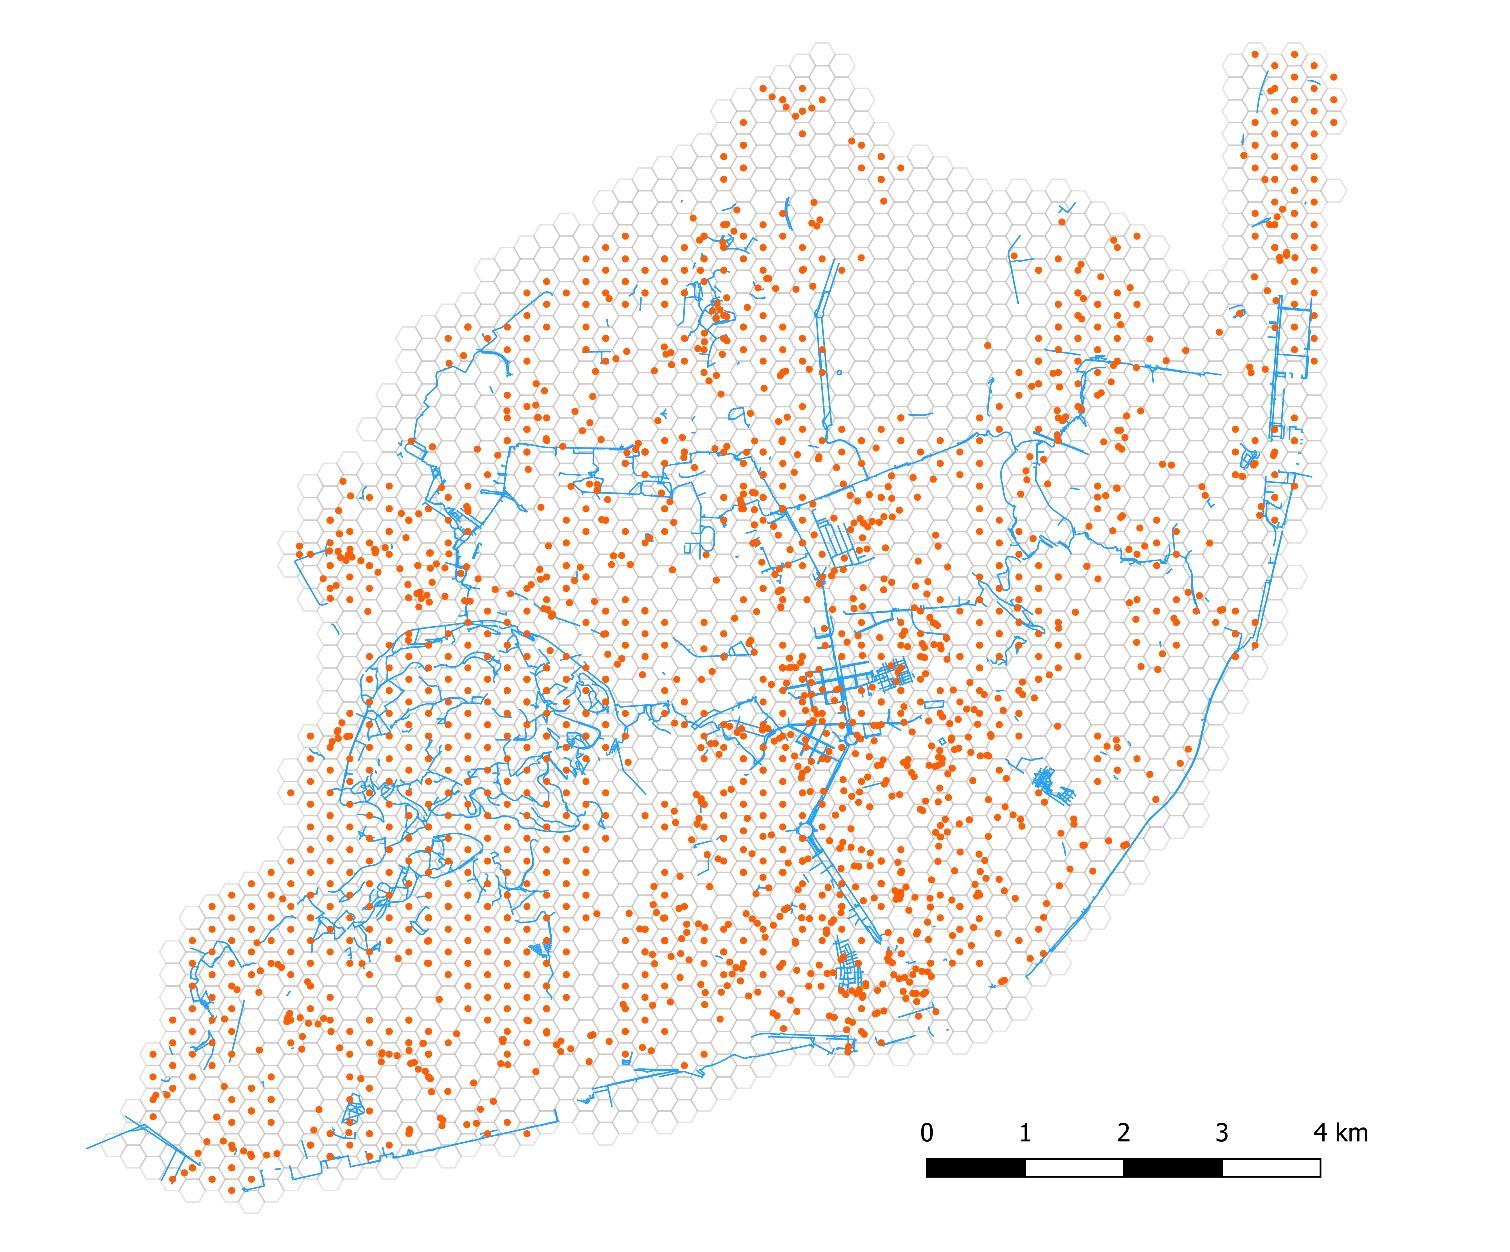
\includegraphics[height=9cm]{appendixA}
		\caption{Destinations, hexagonal grid, and low stress network.}
		\label{appA}
	\end{center}
\end{figure}

\bigskip

\begin{figure}[H]
	\begin{center}
		\includegraphics[height=9cm]{appendixB}
		\caption{Slope percentage for the stress network in Lisbon.}
		\label{appB}
	\end{center}
\end{figure}

\bigskip
%%%%%%%%%%%%%%%%%%%%%%%%%%%%%%%%%%%%%%%%%%
\abbreviations{The following abbreviations are used in this manuscript:\\

\noindent BNA: Bike Network Analysis\\
GIS: Geographic Information Systems\\
PfB: PeopleForBikes
LTS: Level of Traffic Stress\\
OSM: OpenStreetMap\\
CML: Camara Municipal de Lisboa\\
ETRS89: European Terrestrial Reference System 1989\\
DTM: Digital Terrain Model}

%%%%%%%%%%%%%%%%%%%%%%%%%%%%%%%%%%%%%%%%%%
%\bibliographystyle{mdpi}

%=====================================
% References, variant B: external bibliography
%=====================================
\reftitle{References}
\externalbibliography{yes}
\bibliography{Mendeley_BNA}

%%%%%%%%%%%%%%%%%%%%%%%%%%%%%%%%%%%%%%%%%%
\end{document}
